\documentclass[a4paper,TexShade]{class}
\usepackage{graphicx, hyperref}
\usepackage{latexsym, caption, color}
\usepackage{fancyhdr, url}
\usepackage{cite}
\renewcommand\thesection{\arabic{section}}
\urlstyle{rm}


%%%%%%%%%%%%%%%%%%%%%% HEADER %%%%%%%%%%%%%%%%%%%%%%%%%%%
%%%%%%%%%%%%%%%%%%%%%%%%%%%%%%%%%%%%%%%%%%%%%%%%%%%%%%%%%
\SetTitle{\huge{Accumulation Problem}}%
\SetAuthor{Aidela Karamyan\linebreak Ani Sakhlyan\linebreak Sipan Muradyan}%
\SetDepartment{College of Science and Engineering}%
\SetUniversity{American University of Armenia}%
\SetUniversityAddr{Yerevan, Armenia}%
\SetThesisDate{May 9, 2016}%
\SetRequirements{Submitted as partial fulfillment for Communication Networks course}%
\SetCopyright{Copyright \copyright 2016 AUA}%


\begin{document}

\maketitle

\tableofcontents
%\listoftables %
%\listoffigures %


\newpage
\section{Accumulation Problem}

\paragraph{} Accumulation is the "reverse" of broadcasting. Here instead of one vertex passing message to all other vertexes the information flows in the opposite way, all vertexes need to pass their message to one designated vertex. This kind of problem can reflect real life examples when a communication strategy and optimal topology are needed for collecting some sort of data from network participants. Examples of such cases can be collecting sensor data in a network, designing reporting strategy in an organization and more.

\subsection{Problem Definition}
\paragraph{} Given a graph \textit{G} with set of vertexes \textit{V} and edges \textit{E} and a vertex \textit{s $\in$ V}. All the vertexes except \textit{s} contain a distinct piece of information. The communication strategy in which \textit{s}, let's denote it the \textit{server} vertex, will learn the cumulative message from all \textit{v $\in$ V} is called accumulation \cite{book}. 

\paragraph{} Beside the main definition there can be several models worth considering. First important criteria is whether a vertex can simultaneously send and receive messages or can do only one action at a time. This communication models are denoted \textit{2-way} and \textit{1-way} mode respectively. 

\paragraph{} More models can be determined depending on communication buffer criteria, namely how many messages can be sent or received using given connection. Possible models based on this criteria are following:

\bigskip
\begin{enumerate}
\item a vertex \textit{v} can send and receive only 1 message
\item a vertex \textit{v} can send 1 message only, but receive up to \textit{deg(v)} messages
\item a vertex \textit{v} can send up to \textit{deg(v)} messages, but receive only one
\item a vertex \textit{v} can send and receive up to \textit{deg(v)} messages
\end{enumerate}

\bigskip
\paragraph{} In model 2, sine communication line buffer limits the number of passed messages, the more than 1 messages received are received from multiple sources. Similarly in model 3, the more than 1 messages are sent to multiple targets. Remarkable that in model 2 accumulation time is equal to the broadcast time on the same graph, with same vertex taken as the server node and the originator. In model 4 accumulation time is equal to the diameter of the graph, at each time unit all messages stored in the vertex are passed forward so accumulation time is determined by the longest path needed to pass.

Vertex storage space can also be a criteria for model determination, vertex with limited storage cannot receive more messages until freeing some space by sending messages. 


\subsection{Applications} \label{applications}
\paragraph{} An example case where accumulation problem can be useful is a post office transportation topology. Sometimes it is not justified to send one unit directly to the center (center is the analogy of server node), it can be due to transportation costs or traffic considerations. In this kind of situations units need to be accumulated in local spots, than sent to regional spots, than spots of larger size areas and finally to the center.

\paragraph{} Weather station is an example when processing needs to be done on the way to the center. Suppose we have sensors for collecting weather station data. Data from the sensors need to be passed to the middle-ware nodes in the network where it will be filtered. After filtering it can be passed to another layer of middle-ware nodes where some kind of decision making can be done. And finally the processed data will be passed to the center.

\paragraph{} Reporting in organizations is a combination of previous two cases. Obviously it is not practical for everyone to directly report to the higher management, so the reporting is done in levels. Lower level employees report to their direct management, those managers report to higher level management and so on. Also at each level some processing can be done such as making reports based on the received reports.


\subsection{Accumulation on Specific Graphs} \label{accumulation}
\paragraph{} We chose following model for accumulation problem investigation: communication buffer 1-1 mode with unlimited vertex storage buffer and 1-way communication mode. Reason for choosing this model is that it is the most complicated and challenging. Chosen model is reflecting real life problem with hardware limitations, which can occur even with the advanced hardware when huge amounts of data need to be passed as one piece of information. 

\paragraph{} Unlike broadcasting each edge passes multiple pieces of information in different time units, and vertexes can have many states depending on the data stored. So to ease steps description during accumulation process we have developed a \textit{table method} for determining the states of the vertexes at each time unit. Row number defines the states of the vertexes at that time unit, very first row determines states at time 1 and so on. We assume that at time 0 each vertex only has its own message. Column number determines vertex number.

\paragraph{} Now let's discuss accumulation problem on several graph typologies and determine the best possible case to complete the task.

\newpage
\subsubsection{Complete Graph}
\paragraph{} Complete graph is the simplest case for accumulation. With the chosen model it will take \textit{ $(n - 1)$ } time units to pass all messages to the server. Server can receive only one message at each time unit, and it is not meaningful to send message to anywhere other than server since it will not optimize communication anyhow.

\bigskip
\begin{figure}[h]
\centering
\caption{Complete graph} \label{fig:complete}
\caption*{Source: This and all subsequent graph figures are created/generated in our application and saved with Windows screen print feature}
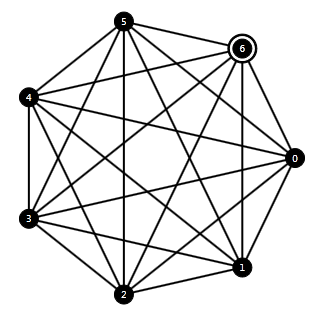
\includegraphics[width=0.6\linewidth ,natwidth=320,natheight=324]{images/complete.png}
\end{figure}

\subsubsection{Star Graph}
In the star graph we have two different server choices. In first case pictured in figure \ref{fig:star} (a), server is the central node. This is similar to complete graph case and accumulation time is \textit{$(n - 1)$}. When we choose one of the star leafs as a server vertex, see figure \ref{fig:star} (b), all messages need to be passed through the center of the star and one at a time only. It will take \textit{ $(n - 2)$ } time units to pass all massages to the center and another \textit{ $(n - 2) + 1$ } for center to pass all the messages including its own message to the server. Overall, the accumulation with worst case server for star graph is \textit{ $2* (n - 2) + 1$ } time units.

\begin{figure}[h]
\centering
\caption{Star graph} \label{fig:star}
   \begin{minipage}{0.49\textwidth}
     \caption*{(a) Central vertex as server}
     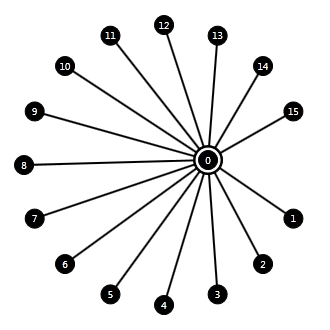
\includegraphics[width=\linewidth ,natwidth=330,natheight=330]{images/star-centre.png}     
   \end{minipage}
   \begin {minipage}{0.49\textwidth}
     \caption*{(b) Leaf vertex as server}
     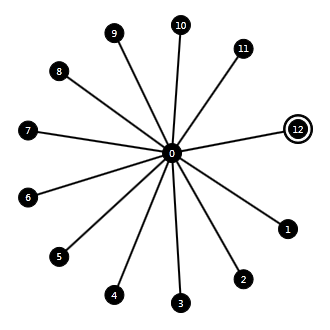
\includegraphics[width=\linewidth ,natwidth=330,natheight=330]{images/star-leaf.png}
   \end{minipage}
\end{figure}


\newpage
\bigskip
\subsubsection{Path Graph}
\paragraph{} In the path graph case the accumulation scheme is different depending on where the server is located. It can be one of the edge vertexes or any vertex up to the center of that path. Odd or even vertexes can also impact the accumulation time.

\paragraph{} Broadcast scheme could be a one similar to the star case, messages are passed sequentially from one end towards the server. That takes \linebreak\textit{ $n * (n - 1) * (n - 2) * ... * 2 * 1$ } time units, which is too long. However turns out that dividing path into pairs of vertexes at each time unit can improve accumulation time. At first time unit vertex closest to the server will send its message, the next two vertexes on the path will also communicate one message towards the server, and so on. 

\bigskip
\begin{figure}[hb]
\centering
\caption{Path graph with central server, even number of vertexes} \label{fig:path-centre-even}
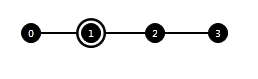
\includegraphics[width=0.49\linewidth ,natwidth=258,natheight=29]{images/path-centre-even.png}
\bigskip
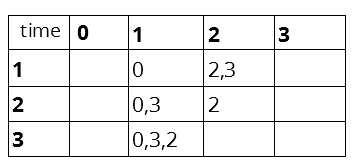
\includegraphics[width=0.49\linewidth ,natwidth=258,natheight=29]{images/path-centre-even-table.png}
\end{figure}


\begin{figure}
\centering
\caption{Path graph with last vertex as server} \label{fig:path-last-even}
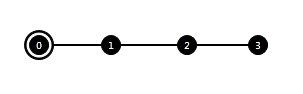
\includegraphics[width=0.5\linewidth ,natwidth=303,natheight=94]{images/path-last-even.png}
\bigskip
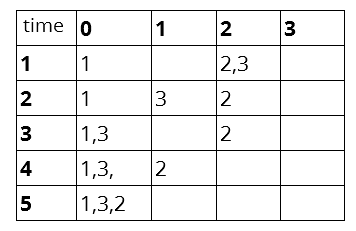
\includegraphics[width=0.6\linewidth ,natwidth=356,natheight=231]{images/path-last-even-table.png}
\end{figure}

\begin{figure}
\centering
\caption{Path graph with central server} \label{fig:path-centre-odd}
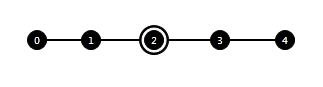
\includegraphics[width=0.55\linewidth ,natwidth=323,natheight=87]{images/path-centre-odd.png}
\bigskip
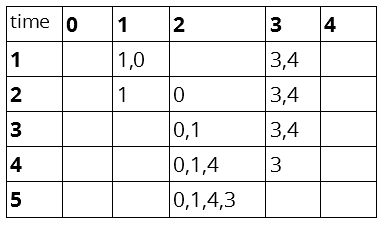
\includegraphics[width=0.6\linewidth ,natwidth=384,natheight=229]{images/path-centre-odd-table.png}
\end{figure}

\newpage
\paragraph{} An example of this scheme with server on one of the last vertexes on an even graph is described in the figure \ref{fig:path-last-even}'s table. Cases when server is not one of the last vertexes is similar, however we deal with 2 paths that need to access the server sequentially. 


\subsubsection{3-ary Tree with Depth 3}
\paragraph{} Tree pictured in figure \ref{fig:tree} is the closest topology to the application examples brought in subsection \ref{applications}. Broadcast scheme for this specific example is following:

\bigskip
\begin{itemize}
\item All leaves transfer their messages to their parent vertexes;\linebreak
server's direct children pass their messages to server  \textit{ : 3} time units
\item Then second level vertexes transfer all their messages to the first level vertexes \textit{ : $ (3 + 1) * 3$}
\item Finally first level vertexes transfer all the collected messages to the server \textit{ : $ (3 + 1) * 3 * 3$}
\item Overall \textit{ $3 + (3 + 1) * 3 + (3 + 1) * 3 * 3 = 51$ } time units
\end{itemize}

\bigskip
\begin{figure}[h]
\centering
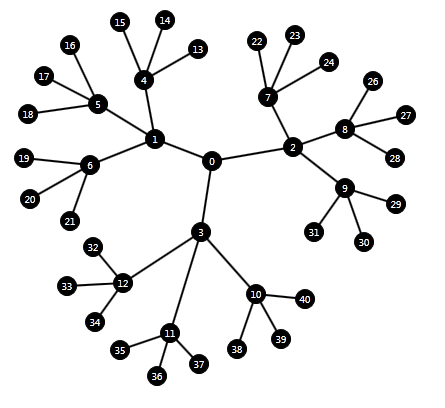
\includegraphics[width=0.8\linewidth ,natwidth=445,natheight=408]{images/3ary-3-tree.png}
\caption{3-ary Tree with Depth 3} \label{fig:tree}
\end{figure}


\newpage
\section{Investigation Program}

\paragraph{} Accumulation is a hard problem in terms of investigation on the paper, compared to broadcasting. Classical broadcasting has one piece of information and in each edge is activated only ones. This makes possible using the paper and pencil method for picturing broadcasting process on the graph itself. 

\paragraph{} Since accumulation has multiple pieces of information the process is radically different. During the accumulation process each edge can have up to \textit{n} (\textit{n} is the number of nodes in the graph) number of pieces of information passed depending on where the edge is located. As a result it is impractical to picture the whole process on the paper in the same way that classical broadcasting is pictured.

\paragraph{} The table method we introduced in subsection \ref{accumulation} makes investigation easier. However, since it lacks visual connection with the graph, method requires to jump your eyes from the graph to the table and back during accumulation process multiple times. Investigation process turns out to be not very productive using this method.

\paragraph{} Given this difficulties, in the scope of this project we developed a new application which will make investigation process easier. It offers following main features

\bigskip
\begin{itemize}
\item conveniently draw and manipulate graphs
\item auto-generate common graph types or random graphs
\item simulate accumulation process steps in an interactive way
\end{itemize}


\bigskip
\subsection{Program Structure} \label{program-structure}

\paragraph{} Our application consists of two parts: command line tool for generating graphs and main application that has all 3 initially planned features. Main application calls command line component internally, however latter can be used as a standalone console application.

\paragraph{} Graph generating command line tool is written in \textit{Python} \cite{python}. Python is a multipurpose high-level programming language. Main reason behind choosing Python for graph generating logic is the \textit{NetworkX} \cite{networkx} library. This library, apart from offering a full-fledged functionality for working with graphs, has a graph generating module supporting more than 50 common graph types and more than 15 different algorithms for generating random graphs \cite{networkx-generators}.

\paragraph{} NetworkX library also has a graph export feature. Exporting is done in \textit{GraphML} format \cite{graphml} which is an XML based text file format for graph representation. This format files are used for passing graphs generated in command line tool to the main application. Since GraphML is a common file format serialization and de-serialization of graphs in this format is made easy with the existing parsing libraries.

\paragraph{} Main application is a Windows application with graphical user interface written in \textit{C\#} \cite{c-sharp} and \textit{Windows Presentation Foundation engine (WPF)} \cite{wpf}. WPF uses \textit{XAML} \cite{xaml} interface markup language which allows to easily create and handle custom graphical components. That is a very important criteria for this kind of applications where components such as graph vertexes and edges are required for drawing and manipulating in a user responsive manner.

\bigskip
\subsection{Graph Generator Tool} \label{graph-generator}

\paragraph{} Command line tool is a graph generating application with easy to use command line interface. Application has 2 commands: "random" and "classic". As mentioned in section \ref{program-structure} NetworkX libary is used for generating graphs and exporting them in GraphML format. 

\bigskip
\begin{figure}[h]
\centering
\caption{Graph generator help output} \label{generator1}
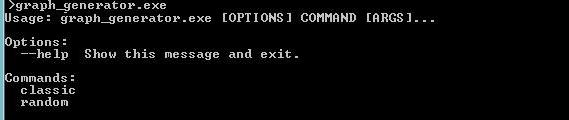
\includegraphics[width=0.9\linewidth ,natwidth=569,natheight=120]{images/generator_screen1.png}
\end{figure}

\paragraph{} "Random" command takes as an argument number of vertexes and generates a random graph. Random graph is generated using \textit{Erd\~{o}s-R\'{e}nyi model} \cite{erdos-renyi}, where graphs is generated with predetermined probability for edge existence. Our program uses 50\% probability by default, this can be changed.

\paragraph{} "Classic" command takes two arguments, the number of vertexes and the type of classical graph. Currently we support path, cycle, star, complete, hypercube and wheel graphs. Code for generating a graph of specific type and exporting it is literally 2 lines of code, so it is only matter of time to add all graph types supported by NetworkX library.

\paragraph{} For example, below is a sample code for generating 20 vertex complete graph with NetworkX library.
\bigskip

\begin{itemize}
\item graph = nx.complete\_graph(20)
\item nx.write\_graphml(graph, './complete\_20.graphml')
\end{itemize}
\bigskip

\begin{figure}[ht]
\centering
\caption{Graph generator help output for "classic" command} \label{generator2}
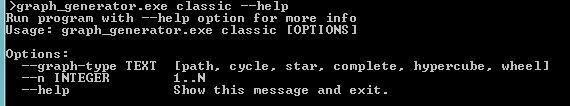
\includegraphics[width=0.9\linewidth ,natwidth=570,natheight=106]{images/generator_screen2.png}
\end{figure}

\begin{figure}[ht]
\centering
\caption{Graph generator "classic" command usage example}
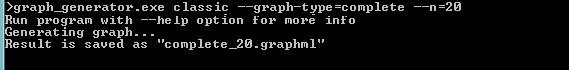
\includegraphics[width=0.9\linewidth ,natwidth=569,natheight=70]{images/generator_screen3.png}
\end{figure}

\paragraph{} Command line program also uses \textit{Click\_} \cite{click} library for designing command line interface in a simple annotated way, that gives flexibility to add more commands or arguments for existing commands. And \textit{PyInstaller} \cite{pyinstaller} application was used to compile Python code to an executable file to make the command line standalone application and call it as a process from the main application.


\bigskip
\newpage
\subsection{Main Application}

\paragraph{} Main application has a white canvas for drawing generated graphs and manual drawing; and a control bar. 

\bigskip
\begin{figure}[h]
\centering
\caption{Main windows screen} \label{fig:main1}
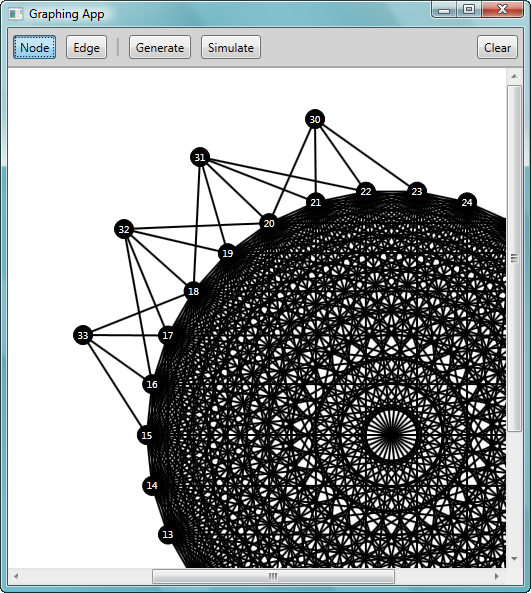
\includegraphics[width=0.8\linewidth ,natwidth=531,natheight=593]{images/main.png}
\end{figure}

\paragraph{} All main features can be accessed with the buttons on the control bar. Toggle buttons on the left corner are manual drawing mode buttons. Two modes are available: node and edge. Both modes can't be active at the same time. When node mode is active mouse left-click on the canvas will create a vertex with sequential id as a label. Id is reset to 0 when all vertexes are deleted. Mouse right-click on the vertex will delete it with all the adjacent edges.

\paragraph{} In the edge mode left-click on the vertex will choose it as a first vertex and change its color to red. After clicking on the second vertex an edge will be drawn connecting those two vertexes. Clicking on the same vertex twice will cancel vertex selection. Mouse right-click works as a delete for edges as well. Mouse left-click and move action on a vertex will re-position it with all the adjacent edges. Delete and re-positioning will work regardless if any of the modes is active.

\paragraph{} Generate button opens windows with generate options. After choosing graph type and number of nodes and pressing "OK" button, main application calls command line graph generator application described in chapter \ref{graph-generator} and gets a GraphML file as a result. 

\paragraph{} GraphML file is parsed using QuickGraph \cite{quick-graph} library's de-serializer and resulting graph is drawn on the canvas. NetworkX library only describes the structure of the graph and does not determine the positions of vertexes, so the coordinates are calculated manually using a simple polygon representation method. \ref{fig:formula} is the formula used for calculating the coordinates.

\bigskip
\begin{figure}[h]
\centering
\caption{Generate options window screen} \label{fig:main2}
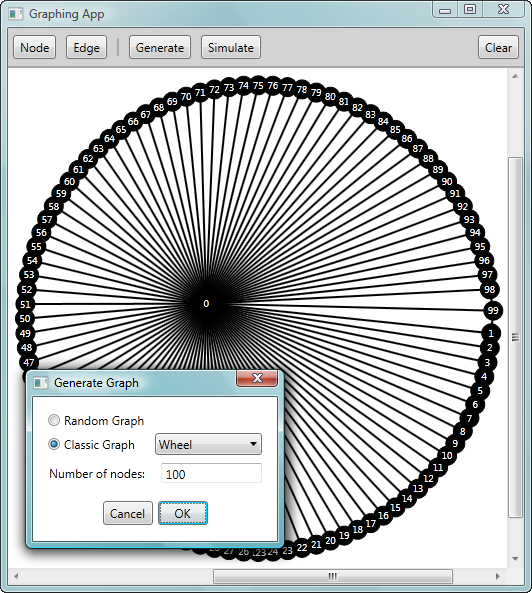
\includegraphics[width=0.8\linewidth ,natwidth=532,natheight=593]{images/main2.png}
\end{figure}


\begin{figure}[h]
\centering
\caption{Vertex coordinate calculation formula} \label{fig:formula}
$
x = centreX + r * \cos(2 * \pi * i / n)
$ \linebreak $
y =  centreY + r * \sin(2 * \pi * i / n)
$ \linebreak $
$ \linebreak $
i = 1\ldots n, n = |V|
$ \linebreak $
r = \min(CanvasWidth, CanvasHeight) / 3
$ \linebreak $
centreX = CanvasWidth / 2
$ \linebreak $
centreY = CanvasHeight / 2
$
\end{figure}


\paragraph{} Graph on the canvas is stored in form of a linked list. Each vertex has an entry with a list of all edges connected to it. Edges in this storage structure are referenced twice to enable deletion of specific vertex with its edged. However in C\# stored edges are actually references to real objects, so in case of extra data kept in the edges there will not be any performance issues. "Clear" button on the right corner of the control bar will clear the canvas and release graph related data.


\paragraph{} The simulator feature is designed for accumulation problem investigation specifically. After clicking on "simulate" button a new window is opened and all buttons on control tab and right-click action become disabled to avoid graph alterations during simulation. The opened window contains a terminal for writing simulation script and control tab with 3 buttons: "start", "next" and "stop". Initially only "start" button is enabled. 

\paragraph{} Script is the code determining the steps and what should be done during simulation. Each line of the code should start with the following string\textit{ "time:"}, \textit{time} is a time-slot sequential number starting from 0. Server vertex should be determined at time 0 with the following line \textit{"0: server \textless- vertex\_id"}, \textit{vertex\_id} is the designated vertex numeric id.
All subsequent lines define how data should be passed. Format is following: 
\bigskip

\textit{number: source\_vertex\_id -\textgreater target\_vertex\_id, source\_vertex\_id -\textgreater target\_vertex\_id...}
\linebreak

\textit{source\_vertex\_id} is the id of the vertex that is passing a piece of message, \textit{target\_vertex\_id} is the id of the vertex that will receive it.

\paragraph{} After writing script and clicking on the "start" button simulation starts and "next", "stop" buttons become enabled. Immediately after clicking "start" button the first line of the script is highlighted. When script line does not have any errors it is highlighted with green color indicating it is the currently executed line of code and user can proceed to the execution of the next line with "next" button. After proceeding the next line becomes highlighted. Highlight color will be red when script line does not have a correct formatting or the vertex ids are not existing vertex ids, in this case "next" button will be disabled. Passing data out of empty vertex and passing data from server vertex are also error cases.

\paragraph{} During the execution of the code's first line, server vertex is visualized on the graph. It gets an extra hollow like circle around main circle. All other script lines are for accumulation data passing visualization. Edges that are used to pass the message and the target vertexes will be colored green during those steps. Hovering over a vertex will show what data it contains.

\paragraph{} "stop" button is for stopping simulation. It is the only option when error is occurred in the script, can also be used for terminating valid code execution. After terminating simulation graph visualization state is also reset.

\bigskip
\begin{figure}[h]
\centering
\caption{Simulate window screen} \label{fig:main3}
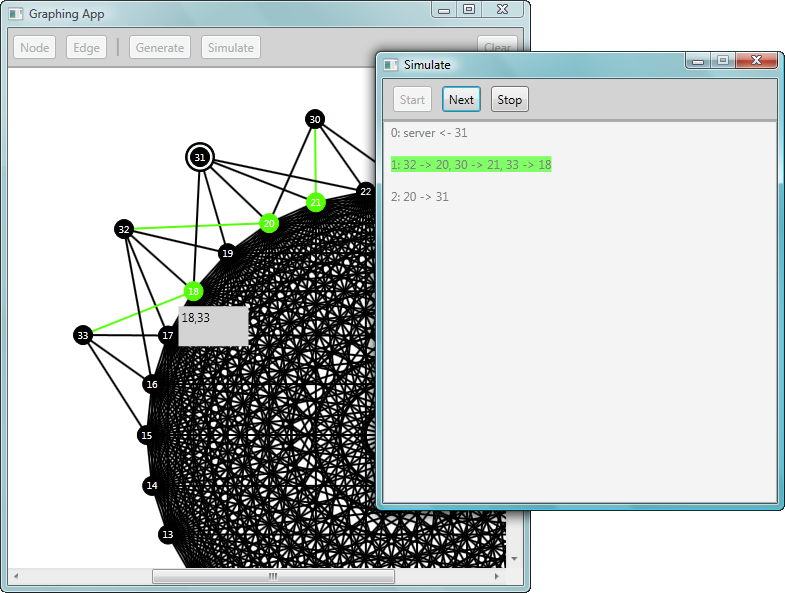
\includegraphics[width=\linewidth ,natwidth=785,natheight=593]{images/main3.png}
\end{figure}


\newpage
\section{Future Work}
\paragraph{} Accumulation is an interesting problem which is not thoroughly investigated for limited options cases. We plan to investigate accumulation problem on more graph typologies and try to determine a general algorithm that will at least complete the task even if not in the best possible time.
And there are multiple features that can be added to the application to make it easier to use and more useful, some of those are
\bigskip

\begin{itemize}
\item Real time syntax warnings in the simulator feature to turn it into a real compiler
\item Size option to the graph generate feature to allow users generate graphs with large amount of vertexes on the canvas, not limited to the screen size
\item Developing a GraphML de-serialization module ourselves to support all graph types generated by NetworkX library and replacing currently used de-serializer
\item Implementing more graph layout algorithms 
\item Exporting graphs in GraphML and .png image formats
\end{itemize}


\bibHeading{\textbf{References}}
\bibliography{resources}
\bibliographystyle{unsrt}


\end{document} 
